
\documentclass[border=10pt, 12pt]{standalone}
\usepackage[svgnames]{xcolor}
\usepackage{amsmath}
\usepackage{pgfplots}
\pgfplotsset{compat=newest}
\usepackage[sfdefault]{FiraSans}
\usepackage{FiraMono}
\renewcommand*\familydefault{\sfdefault}
\begin{document}
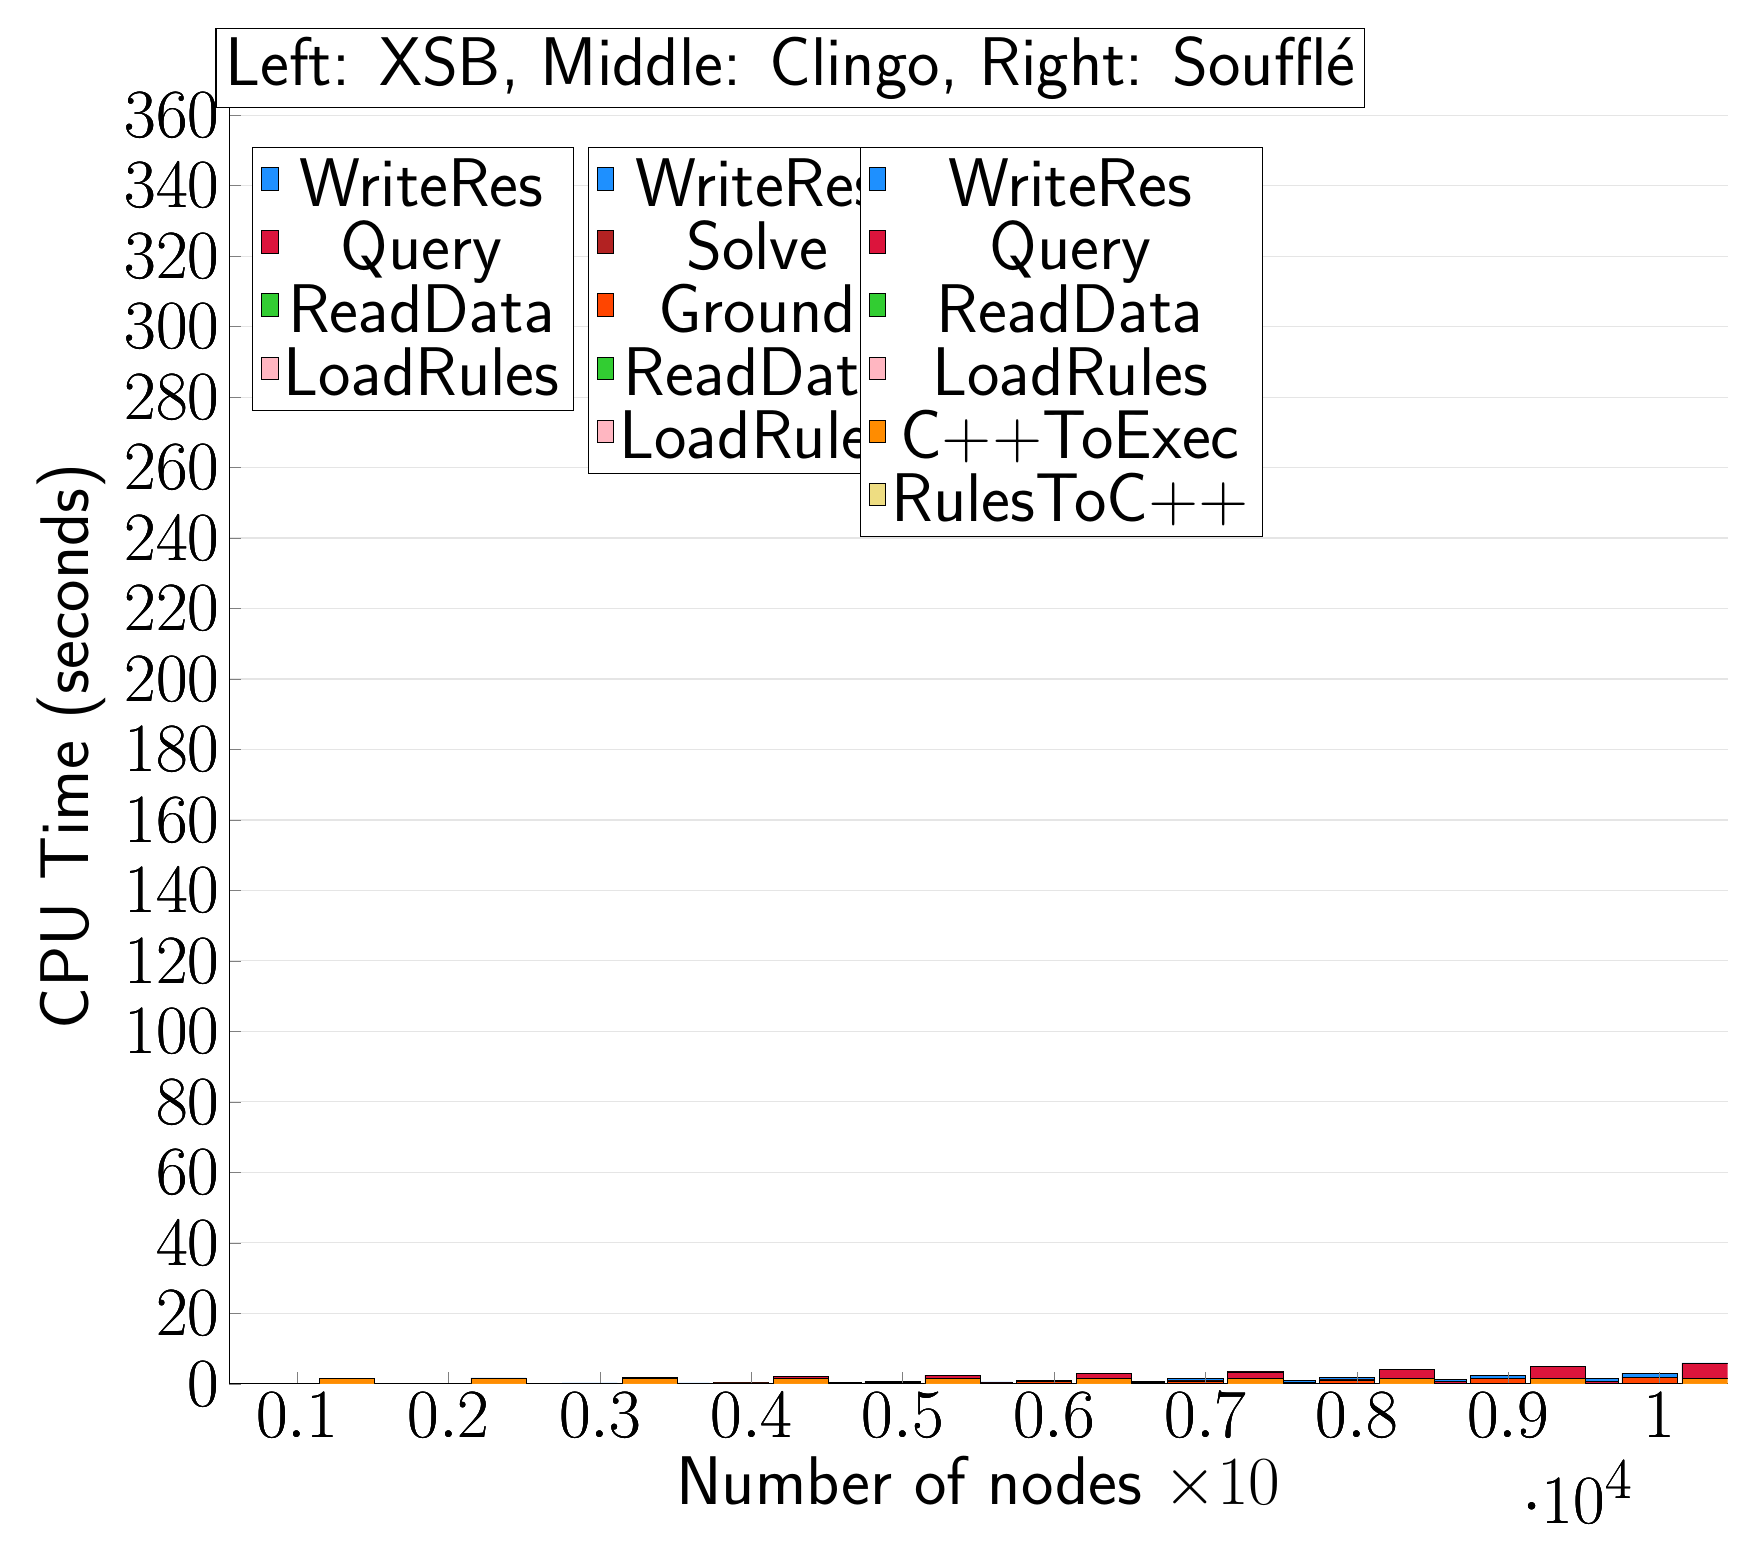
\begin{tikzpicture}
                        \begin{axis}[bar shift=-25pt, 
   ybar stacked,
   width=1.7\textwidth,
   bar width=0.7cm,
   ymajorgrids, tick align=inside,
   major grid style={draw=gray!20},
   xtick=data,
   ymin=0, ymax=361.9108,
   axis x line*=bottom,
   axis y line*=left,
   enlarge x limits=0.05,
   legend style={
       at={(0.23, 0.97)},
       anchor=north east,
       legend columns=1,
       font=\Huge,
   },
   ylabel={CPU Time (seconds)},
   xlabel={Number of nodes $\times 10$},
   label style={font=\Huge},
   tick label style={font=\Huge},
]
\addlegendimage{fill=DodgerBlue, draw=black, line width=0.2pt}
\addlegendentry{WriteRes}
\addlegendimage{fill=Crimson, draw=black, line width=0.2pt}
\addlegendentry{Query}
\addlegendimage{fill=LimeGreen, draw=black, line width=0.2pt}
\addlegendentry{ReadData}
\addlegendimage{fill=LightPink, draw=black, line width=0.2pt}
\addlegendentry{LoadRules}
\addplot +[fill=LightPink, draw=black, line width=0.2pt] coordinates {
(1000, 0.0005528000000000002)
(2000, 0.0005491999999999996)
(3000, 0.0005538000000000002)
(4000, 0.0005511999999999997)
(5000, 0.0005477999999999995)
(6000, 0.0005483999999999995)
(7000, 0.0005494000000000001)
(8000, 0.0005531999999999999)
(9000, 0.0005489999999999998)
(10000, 0.0005497999999999996)
};
\addplot +[fill=LimeGreen, draw=black, line width=0.2pt] coordinates {
(1000, 0.0009484000000000001)
(2000, 0.0018444)
(3000, 0.0026932)
(4000, 0.0035306000000000005)
(5000, 0.004449)
(6000, 0.0053036)
(7000, 0.006144599999999999)
(8000, 0.007009400000000001)
(9000, 0.007875199999999999)
(10000, 0.0087764)
};
\addplot +[fill=Crimson, draw=black, line width=0.2pt] coordinates {
(1000, 0.0065294)
(2000, 0.028048200000000002)
(3000, 0.06320440000000001)
(4000, 0.1112376)
(5000, 0.17834099999999997)
(6000, 0.24581240000000001)
(7000, 0.3431778)
(8000, 0.4432956)
(9000, 0.6014798000000001)
(10000, 0.712163)
};
\addplot +[fill=DodgerBlue, draw=black, line width=0.2pt] coordinates {
(1000, 0.0084332)
(2000, 0.033774200000000004)
(3000, 0.07453900000000001)
(4000, 0.134281)
(5000, 0.20667839999999998)
(6000, 0.30165999999999993)
(7000, 0.40596920000000003)
(8000, 0.5347396)
(9000, 0.6697424)
(10000, 0.8312522)
};
\end{axis}

\begin{axis}[bar shift=-3.7pt, 
   ybar stacked,
   width=1.7\textwidth,
   bar width=0.7cm,
   ymajorgrids, tick align=inside,
   major grid style={draw=none},
   xtick=data,
   ymin=0, ymax=361.9108,
   axis x line*=none,
   axis y line*=none,
   enlarge x limits=0.05,
   legend style={
       at={(0.454, 0.97)},
       anchor=north east,
       legend columns=1,
       font=\Huge,
   },
   label style={font=\Huge},
   tick label style={font=\Huge},
]
\addlegendimage{fill=DodgerBlue, draw=black, line width=0.2pt}
\addlegendentry{WriteRes}
\addlegendimage{fill=FireBrick, draw=black, line width=0.2pt}
\addlegendentry{Solve}
\addlegendimage{fill=OrangeRed, draw=black, line width=0.2pt}
\addlegendentry{Ground}
\addlegendimage{fill=LimeGreen, draw=black, line width=0.2pt}
\addlegendentry{ReadData}
\addlegendimage{fill=LightPink, draw=black, line width=0.2pt}
\addlegendentry{LoadRules}
\addplot +[fill=LightPink, draw=black, line width=0.2pt] coordinates {
(1000, 0.0)
(2000, 0.0)
(3000, 0.0)
(4000, 0.0)
(5000, 0.0)
(6000, 0.0)
(7000, 0.0)
(8000, 0.0)
(9000, 0.0)
(10000, 0.0)
};
\addplot +[fill=LimeGreen, draw=black, line width=0.2pt] coordinates {
(1000, 0.0)
(2000, 0.0)
(3000, 0.0040000000000000036)
(4000, 0.010000000000000009)
(5000, 0.010000000000000009)
(6000, 0.01200000000000001)
(7000, 0.010000000000000009)
(8000, 0.020000000000000018)
(9000, 0.020000000000000018)
(10000, 0.020000000000000018)
};
\addplot +[fill=OrangeRed, draw=black, line width=0.2pt] coordinates {
(1000, 0.020000000000000018)
(2000, 0.062)
(3000, 0.14400000000000002)
(4000, 0.252)
(5000, 0.4080000000000001)
(6000, 0.606)
(7000, 0.8460000000000001)
(8000, 1.108)
(9000, 1.4259999999999997)
(10000, 1.802)
};
\addplot +[fill=FireBrick, draw=black, line width=0.2pt] coordinates {
(1000, 0.0)
(2000, 0.006000000000000005)
(3000, 0.0020000000000000018)
(4000, 0.012000000000000009)
(5000, 0.020000000000000018)
(6000, 0.020000000000000018)
(7000, 0.02600000000000003)
(8000, 0.041999999999999815)
(9000, 0.05800000000000004)
(10000, 0.062000000000000055)
};
\addplot +[fill=DodgerBlue, draw=black, line width=0.2pt] coordinates {
(1000, 0.010000000000000009)
(2000, 0.03999999999999998)
(3000, 0.118)
(4000, 0.17999999999999994)
(5000, 0.2779999999999999)
(6000, 0.4200000000000001)
(7000, 0.5699999999999998)
(8000, 0.7400000000000002)
(9000, 0.916)
(10000, 1.1560000000000001)
};
\end{axis}

\begin{axis}[bar shift=18pt, 
   ybar stacked,
   width=1.7\textwidth,
   bar width=0.7cm,
   ymajorgrids, tick align=inside,
   major grid style={draw=none},
   xtick=data,
   ymin=0, ymax=361.9108,
   axis x line*=none,
   axis y line*=none,
   enlarge x limits=0.05,
   legend style={
       at={(0.69, 0.97)},
       anchor=north east,
       legend columns=1,
       font=\Huge,
   },
   label style={font=\Huge},
   tick label style={font=\Huge},
]
\addlegendimage{fill=DodgerBlue, draw=black, line width=0.2pt}
\addlegendentry{WriteRes}
\addlegendimage{fill=Crimson, draw=black, line width=0.2pt}
\addlegendentry{Query}
\addlegendimage{fill=LimeGreen, draw=black, line width=0.2pt}
\addlegendentry{ReadData}
\addlegendimage{fill=LightPink, draw=black, line width=0.2pt}
\addlegendentry{LoadRules}
\addlegendimage{fill=DarkOrange, draw=black, line width=0.2pt}
\addlegendentry{C++ToExec}
\addlegendimage{fill=LightGoldenrod, draw=black, line width=0.2pt}
\addlegendentry{RulesToC++}
\addplot +[fill=LightGoldenrod, draw=black, line width=0.2pt] coordinates {
(1000, 0.004000000000000001)
(2000, 0.006000000000000001)
(3000, 0.008000000000000002)
(4000, 0.006000000000000001)
(5000, 0.010000000000000002)
(6000, 0.006000000000000001)
(7000, 0.0020000000000000005)
(8000, 0.006000000000000001)
(9000, 0.0020000000000000005)
(10000, 0.004000000000000001)
};
\addplot +[fill=DarkOrange, draw=black, line width=0.2pt] coordinates {
(1000, 1.482)
(2000, 1.482)
(3000, 1.4520000000000002)
(4000, 1.4540000000000002)
(5000, 1.4520000000000004)
(6000, 1.47)
(7000, 1.4679999999999997)
(8000, 1.4480000000000002)
(9000, 1.472)
(10000, 1.4780000000000002)
};
\addplot +[fill=LightPink, draw=black, line width=0.2pt] coordinates {
(1000, 0.0001464)
(2000, 0.000153)
(3000, 9.8e-05)
(4000, 4.78e-05)
(5000, 0.00011800000000000001)
(6000, 0.00017959999999999997)
(7000, 0.0001672)
(8000, 0.0001454)
(9000, 0.000149)
(10000, 0.0001656)
};
\addplot +[fill=LimeGreen, draw=black, line width=0.2pt] coordinates {
(1000, 0.0043524)
(2000, 0.0078052)
(3000, 0.0071806)
(4000, 0.008126600000000001)
(5000, 0.013594400000000001)
(6000, 0.020339199999999998)
(7000, 0.0212142)
(8000, 0.0206714)
(9000, 0.0251372)
(10000, 0.028243399999999995)
};
\addplot +[fill=Crimson, draw=black, line width=0.2pt] coordinates {
(1000, 0.050414)
(2000, 0.1532508)
(3000, 0.32878299999999994)
(4000, 0.6108724000000001)
(5000, 0.9566014)
(6000, 1.4009440000000002)
(7000, 1.9211940000000003)
(8000, 2.554812)
(9000, 3.3841900000000003)
(10000, 4.233051999999999)
};
\addplot +[fill=DodgerBlue, draw=black, line width=0.2pt] coordinates {
(1000, 0.0027549999999999996)
(2000, 0.0088114)
(3000, 0.0198364)
(4000, 0.034567600000000004)
(5000, 0.05414100000000001)
(6000, 0.0772374)
(7000, 0.10429379999999999)
(8000, 0.1370336)
(9000, 0.1755298)
(10000, 0.212608)
};
\end{axis}


\node[anchor=south, draw, fill=white] at (rel axis cs:0.42,1) {\Huge Left: XSB, Middle: Clingo, Right: Soufflé};
\end{tikzpicture}
\end{document}
                    